\documentclass[border=10pt]{standalone}

% Compilacao: pdflatex -interaction=nonstopmode -halt-on-error diagrama_protecao.tex
% PNG 300 dpi: pdftoppm -png -r 300 -singlefile diagrama_protecao.pdf images/diagrama_protecao
\usepackage[T1]{fontenc}
\usepackage[utf8]{inputenc}
\usepackage{helvet}
\renewcommand{\familydefault}{\sfdefault}
\usepackage{xcolor}
\usepackage{tikz}
\usepackage{circuitikz}
\usetikzlibrary{arrows.meta,positioning,shapes,calc}

% Cores da referencia.
\definecolor{tcblue}{RGB}{43,114,196}
\definecolor{tripred}{RGB}{217,56,58}
\definecolor{relaybg}{RGB}{254,250,230}
\definecolor{relayborder}{RGB}{184,134,11}
\definecolor{legendgray}{RGB}{180,180,180}

\tikzset{
  power/.style={draw=black,line width=1.1pt,line cap=butt},
  bus/.style={draw=black,ultra thick,line width=2.5pt,line cap=butt},
  tc signal/.style={draw=tcblue,line width=.7pt,
    preaction={draw=white,line width=2.2pt}},
  trip/.style={draw=tripred,dashed,thick,dash pattern=on 4pt off 2.5pt},
  breaker/.style={draw=black,fill=white,line width=1.1pt,
    minimum width=8.6mm,minimum height=8.6mm,inner sep=0pt,
    font=\fontsize{8}{9}\selectfont},
  future breaker/.style={breaker,dashed,dash pattern=on 4pt off 2.5pt},
  current transformer/.style={rectangle,draw=none,fill=none,
    minimum width=8.4mm,minimum height=5.6mm,inner sep=0pt},
  % Enrolamento de dois arcos conforme a referencia elementos.jpg.
  % Simbolo inserido no eixo do condutor, sem deslocamento lateral.
  pics/tc winding/.style={code={%
    \draw[white,line width=2.4pt] (0,-.28)--(0,.28);
    \draw[power] (0,.28)
      arc[start angle=90,end angle=270,radius=.14]
      arc[start angle=90,end angle=270,radius=.14];
    \draw[power] (0,.28)--(.16,.28)
                 (0,-.28)--(.16,-.28);
  }},
  winding/.style={circle,draw=black,fill=white,line width=1.15pt,
    minimum size=14.8mm,inner sep=0pt,font=\fontsize{10}{11}\selectfont},
  relay/.style={draw=relayborder,fill=relaybg,line width=.85pt,
    rounded corners=1.2pt,inner sep=0pt},
  relay title/.style={font=\bfseries\fontsize{9}{11}\selectfont,align=center},
  relay text/.style={font=\fontsize{9}{11}\selectfont,align=center},
  equipment label/.style={font=\bfseries\fontsize{8.5}{10}\selectfont},
  data label/.style={font=\fontsize{8}{9.5}\selectfont,align=left},
  trip label/.style={text=tripred,font=\fontsize{7}{8}\selectfont,
    align=center,fill=white,inner sep=1pt},
  legend text/.style={font=\fontsize{8}{10}\selectfont,anchor=west},
  junction/.style={circle,fill=tcblue,draw=none,minimum size=2pt,inner sep=0pt},
  trip junction/.style={circle,fill=tripred,draw=none,minimum size=2pt,inner sep=0pt}
}

% Simbolos nomeados: os pontos east/west permitem terminar cada sinal
% na borda do equipamento, sem atravessar seu texto ou seu interior.
\newcommand{\CircuitBreaker}[4][]{%
  \node[breaker,#1] (#2) at (#3,#4) {D};
}
% Orientacao opcional: 1 para sinal a direita; -1 para sinal a esquerda.
\newcommand{\CurrentTransformer}[4][1]{%
  \node[current transformer] (#2) at (#3,#4) {};
  \begin{scope}[shift={(#3,#4)},xscale=#1]
    \pic[transform shape] {tc winding};
    % Saida azul no centro do TC, alinhada ao seu eixo horizontal.
    \draw[tc signal] (0,0)--(.42,0);
  \end{scope}
}
\newcommand{\Earth}[2]{%
  \draw[power] (#1,#2) -- ++(0,-.30);
  \draw[power] (#1-.48,#2-.30) -- (#1+.48,#2-.30);
  \draw[power] (#1-.32,#2-.47) -- (#1+.32,#2-.47);
  \draw[power] (#1-.16,#2-.64) -- (#1+.16,#2-.64);
}

\begin{document}
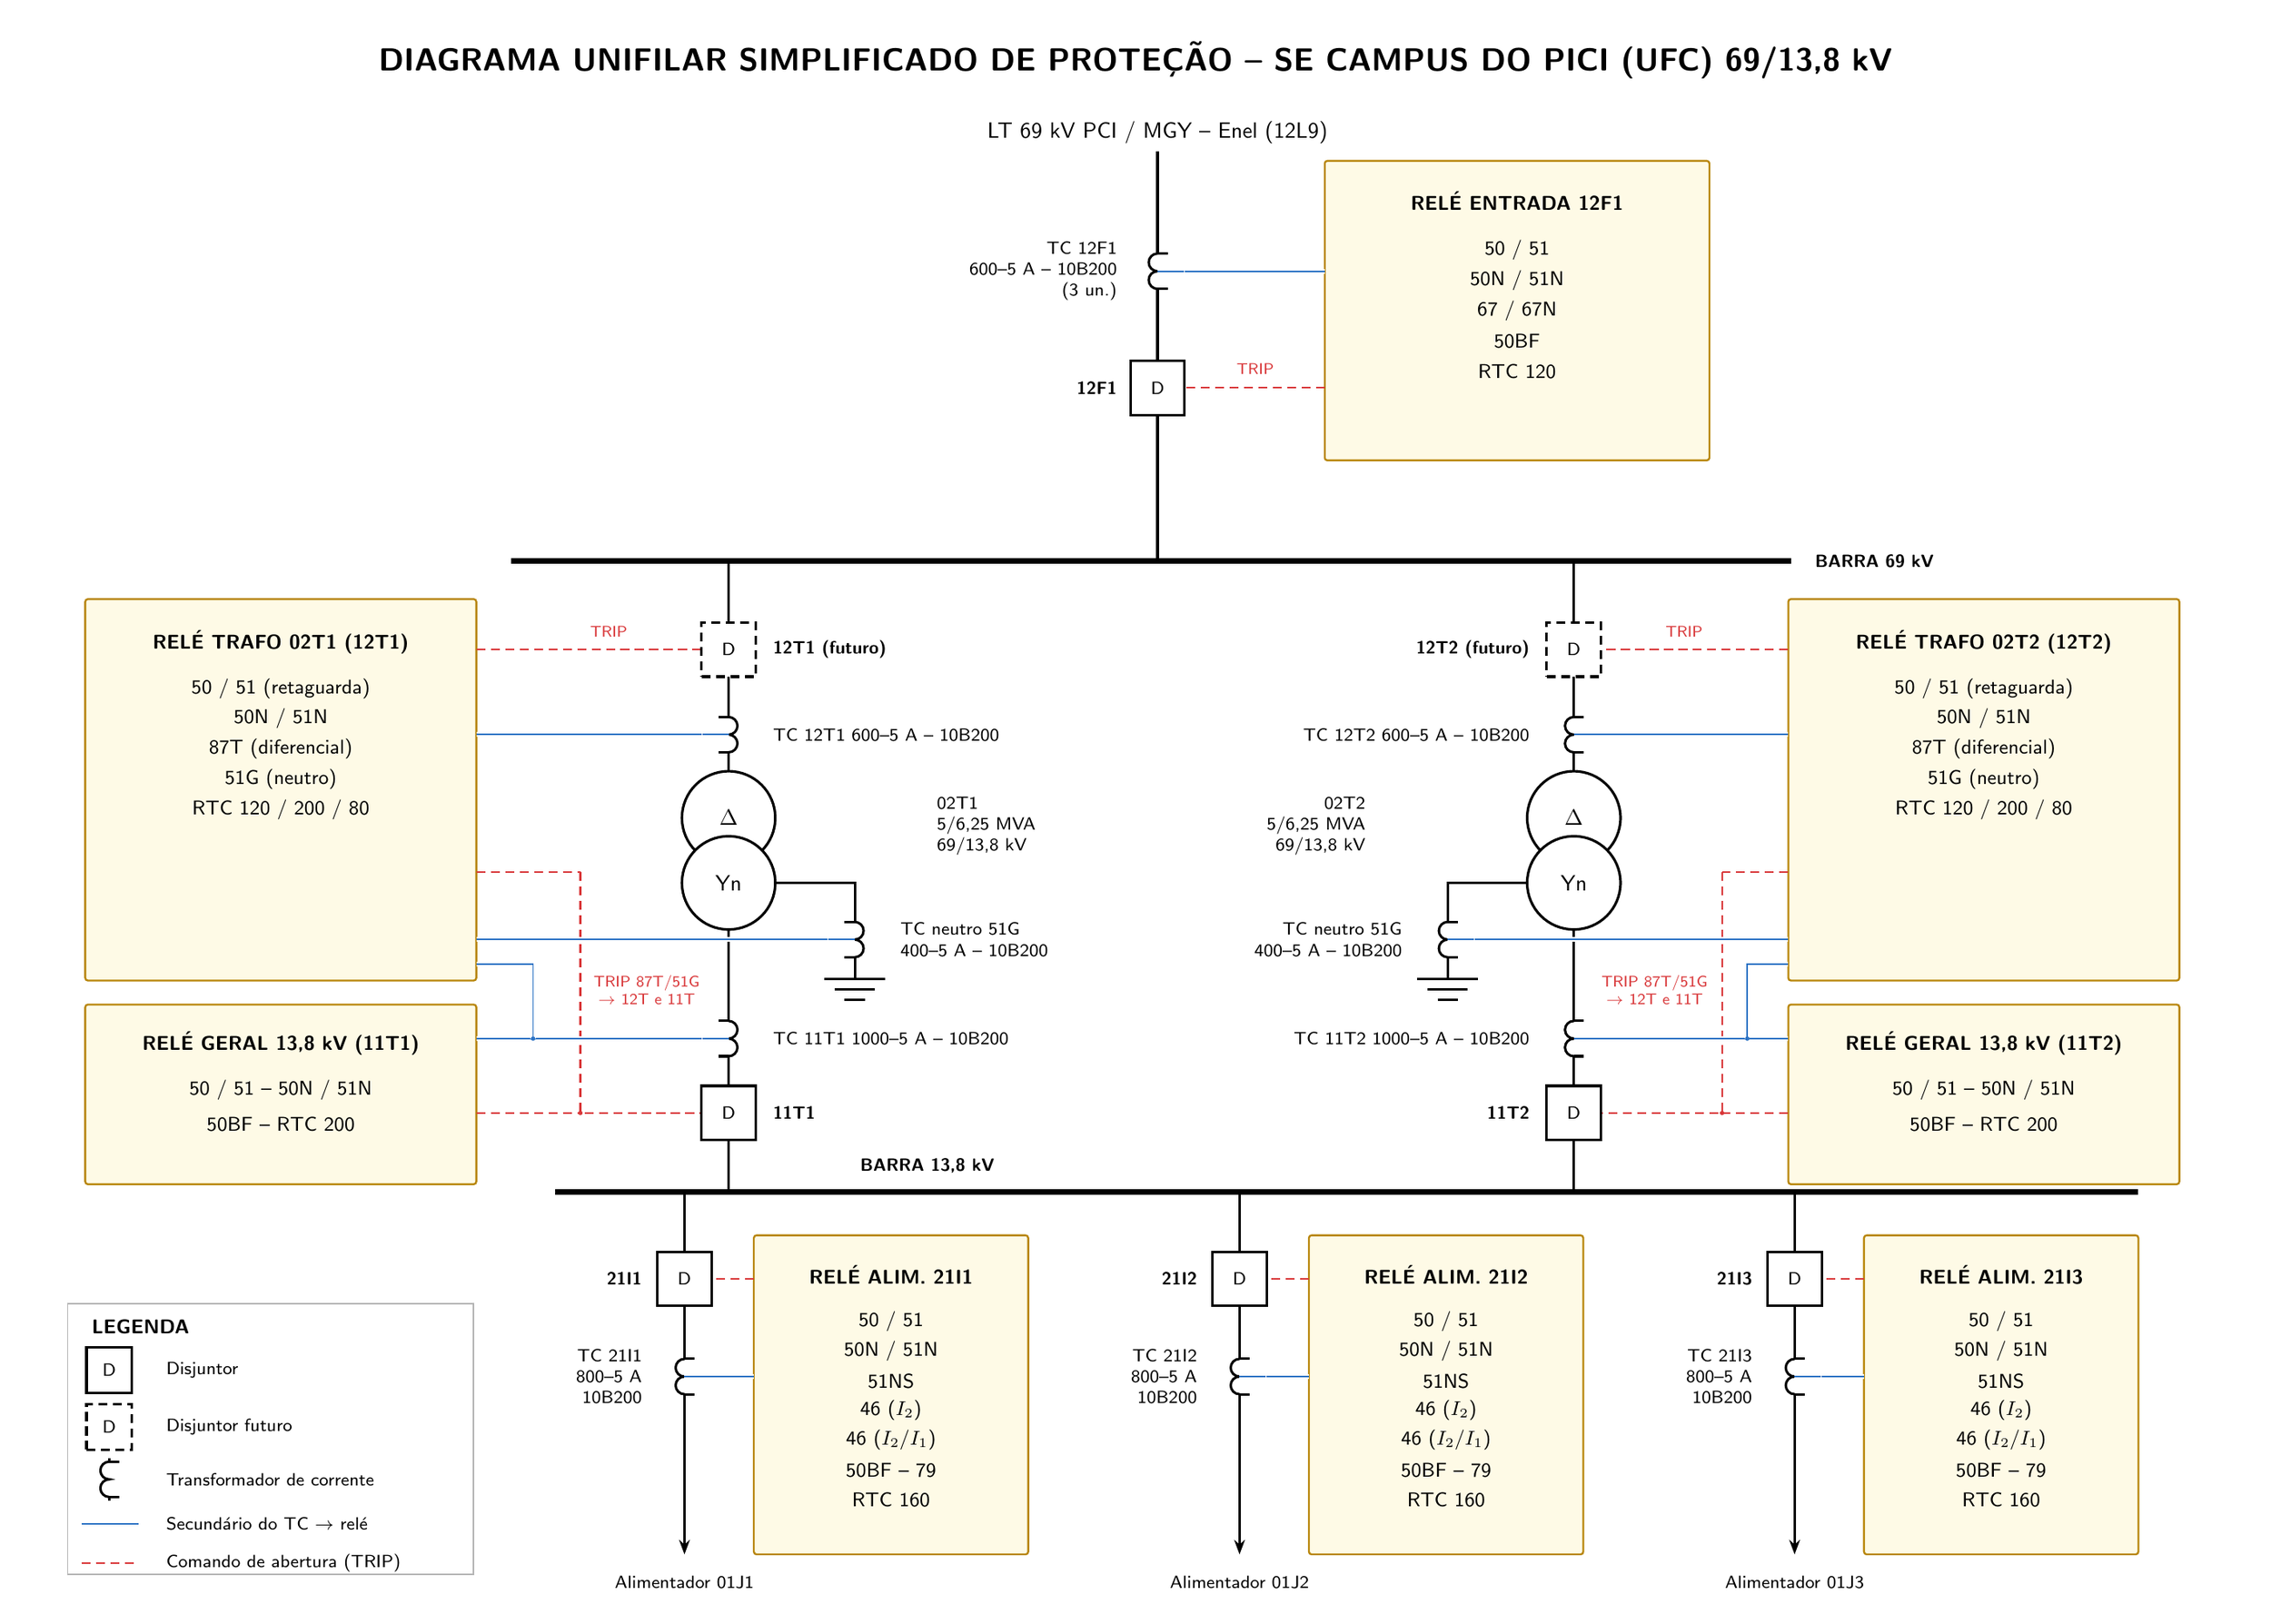
\begin{tikzpicture}[x=1cm,y=1cm,font=\fontsize{9}{11}\selectfont]
  % Folha branca, com proporcao e distribuicao proximas da referencia.
  \path[use as bounding box] (0,-.45) rectangle (35.3,24.6);

  \node[font=\bfseries\fontsize{14}{17}\selectfont,align=center]
    at (17.65,24.0)
    {DIAGRAMA UNIFILAR SIMPLIFICADO DE PROTEÇÃO -- SE CAMPUS DO PICI (UFC) 69/13,8 kV};

  % ================================================================
  % 1. POTENCIA: entrada de linha, barras e dois bays de transformacao.
  % ================================================================
  \node[font=\fontsize{10}{12}\selectfont] at (18,22.85)
    {LT 69 kV PCI / MGY -- Enel (12L9)};
  \draw[power] (18,22.55) -- (18,16.05);
  \draw[bus] (7.75,16.05) -- (28.05,16.05);
  \node[anchor=west,equipment label] at (28.3,16.05) {BARRA 69 kV};

  \foreach \x in {11.2,24.6}{\draw[power] (\x,16.05) -- (\x,6.05);}
  \draw[bus] (8.45,6.05) -- (33.55,6.05);
  \node[anchor=south,equipment label] at (14.35,6.23) {BARRA 13,8 kV};

  % Neutros fisicos dos enrolamentos Yn, com TC em serie no aterramento.
  \draw[power] (11.2,10.95) -- (13.2,10.95) -- (13.2,9.73);
  \draw[power] (24.6,10.95) -- (22.6,10.95) -- (22.6,9.73);
  \Earth{13.2}{9.73}
  \Earth{22.6}{9.73}

  % Alimentadores: condutores continuos sob os simbolos brancos.
  \foreach \x in {10.5,19.3,28.1}{
    \draw[power,-{Stealth[length=2.3mm,width=1.7mm]}]
      (\x,6.05) -- (\x,.30);
  }

  % ================================================================
  % 2. CAIXAS DOS RELES.
  % ================================================================
  \draw[relay] (20.65,17.65) rectangle (26.75,22.40);
  \node[relay title] at (23.70,21.77) {RELÉ ENTRADA 12F1};
  \node[relay text] at (23.70,20.98) {50 / 51};
  \node[relay text] at (23.70,20.50) {50N / 51N};
  \node[relay text] at (23.70,20.02) {67 / 67N};
  \node[relay text] at (23.70,19.54) {50BF};
  \node[relay text] at (23.70,19.06) {RTC 120};

  \foreach \left/\right/\center/\n in {1.0/7.2/4.1/1,28.0/34.2/31.1/2}{
    \draw[relay] (\left,9.40) rectangle (\right,15.45);
    \node[relay title] at (\center,14.77) {RELÉ TRAFO 02T\n\ (12T\n)};
    \node[relay text] at (\center,14.03) {50 / 51 (retaguarda)};
    \node[relay text] at (\center,13.55) {50N / 51N};
    \node[relay text] at (\center,13.07) {87T (diferencial)};
    \node[relay text] at (\center,12.59) {51G (neutro)};
    \node[relay text] at (\center,12.11) {RTC 120 / 200 / 80};

    \draw[relay] (\left,6.17) rectangle (\right,9.02);
    \node[relay title] at (\center,8.40) {RELÉ GERAL 13,8 kV (11T\n)};
    \node[relay text] at (\center,7.66) {50 / 51 -- 50N / 51N};
    \node[relay text] at (\center,7.12) {50BF -- RTC 200};
  }

  \foreach \left/\right/\center/\n in {
    11.60/15.95/13.775/1,20.40/24.75/22.575/2,29.20/33.55/31.375/3}{
    \draw[relay] (\left,.30) rectangle (\right,5.36);
    \node[relay title] at (\center,4.73) {RELÉ ALIM. 21I\n};
    \node[relay text] at (\center,3.99) {50 / 51};
    \node[relay text] at (\center,3.52) {50N / 51N};
    \node[relay text] at (\center,3.05) {51NS};
    \node[relay text] at (\center,2.58) {46 ($I_2$)};
    \node[relay text] at (\center,2.11) {46 ($I_2/I_1$)};
    \node[relay text] at (\center,1.64) {50BF -- 79};
    \node[relay text] at (\center,1.17) {RTC 160};
  }

  % ================================================================
  % 3. EQUIPAMENTOS E RESPECTIVOS IDENTIFICADORES.
  % ================================================================
  \CurrentTransformer{TC12F1}{18}{20.65}
  \CircuitBreaker{DJ12F1}{18}{18.80}
  \node[anchor=east,data label,align=right] at (17.48,20.65)
    {TC 12F1\\600--5 A -- 10B200\\(3 un.)};
  \node[anchor=east,equipment label] at (17.48,18.80) {12F1};

  % Transformador 02T1.
  \CircuitBreaker[future breaker]{DJ12T1}{11.2}{14.65}
  \CurrentTransformer[-1]{TC12T1}{11.2}{13.30}
  \node[winding] (T1delta) at (11.2,11.98) {$\Delta$};
  \node[winding] (T1star) at (11.2,10.95) {Yn};
  \CurrentTransformer[-1]{TCN1}{13.2}{10.05}
  \CurrentTransformer[-1]{TC11T1}{11.2}{8.48}
  \CircuitBreaker{DJ11T1}{11.2}{7.30}
  \node[anchor=west,equipment label] at (11.78,14.65) {12T1 (futuro)};
  \node[anchor=west,data label] at (11.78,13.30) {TC 12T1 600--5 A -- 10B200};
  \node[anchor=west,data label] at (14.38,11.85)
    {02T1\\5/6,25 MVA\\69/13,8 kV};
  \node[anchor=west,data label] at (13.80,10.05)
    {TC neutro 51G\\400--5 A -- 10B200};
  \node[anchor=west,data label] at (11.78,8.48) {TC 11T1 1000--5 A -- 10B200};
  \node[anchor=west,equipment label] at (11.78,7.30) {11T1};

  % Transformador 02T2, espelhado em relacao ao primeiro bay.
  \CircuitBreaker[future breaker]{DJ12T2}{24.6}{14.65}
  \CurrentTransformer{TC12T2}{24.6}{13.30}
  \node[winding] (T2delta) at (24.6,11.98) {$\Delta$};
  \node[winding] (T2star) at (24.6,10.95) {Yn};
  \CurrentTransformer{TCN2}{22.6}{10.05}
  \CurrentTransformer{TC11T2}{24.6}{8.48}
  \CircuitBreaker{DJ11T2}{24.6}{7.30}
  \node[anchor=east,equipment label] at (24.02,14.65) {12T2 (futuro)};
  \node[anchor=east,data label] at (24.02,13.30) {TC 12T2 600--5 A -- 10B200};
  \node[anchor=east,data label,align=right] at (21.42,11.85)
    {02T2\\5/6,25 MVA\\69/13,8 kV};
  \node[anchor=east,data label,align=right] at (22.00,10.05)
    {TC neutro 51G\\400--5 A -- 10B200};
  \node[anchor=east,data label] at (24.02,8.48) {TC 11T2 1000--5 A -- 10B200};
  \node[anchor=east,equipment label] at (24.02,7.30) {11T2};

  \foreach \x/\n in {10.5/1,19.3/2,28.1/3}{
    \CircuitBreaker{DJ21I\n}{\x}{4.67}
    \CurrentTransformer{TC21I\n}{\x}{3.12}
    \node[anchor=east,equipment label] at (\x-.55,4.67) {21I\n};
    \node[anchor=east,data label,align=right] at (\x-.55,3.12)
      {TC 21I\n\\800--5 A\\10B200};
    \node[anchor=north,font=\fontsize{8.5}{10}\selectfont] at (\x,.08)
      {Alimentador 01J\n};
  }

  % ================================================================
  % 4. TRIP: vermelho tracejado; saidas independentes para 12T e 11T.
  % ================================================================
  \draw[trip] (20.65,18.80) -- (DJ12F1.east);
  \node[trip label] at (19.55,19.10) {TRIP};

  % 02T1: contatos de saida independentes do rele de trafo comandam
  % 12T1 e 11T1. A saida do rele geral comanda somente 11T1.
  \draw[trip] (7.2,14.65) -- (DJ12T1.west);
  \draw[trip] (7.2,11.12) -- (8.85,11.12);
  \draw[trip] (8.85,11.12) -- (8.85,7.30) -- (DJ11T1.west);
  \draw[trip] (7.2,7.30) -- (8.85,7.30);
  \node[trip junction] at (8.85,7.30) {};
  \node[trip label] at (9.30,14.94) {TRIP};
  \node[trip label,text width=1.72cm] at (9.90,9.25)
    {TRIP 87T/51G\\$\rightarrow$ 12T e 11T};

  % 02T2: roteamento simetrico.
  \draw[trip] (28.0,14.65) -- (DJ12T2.east);
  \draw[trip] (28.0,11.12) -- (26.95,11.12);
  \draw[trip] (26.95,11.12) -- (26.95,7.30) -- (DJ11T2.east);
  \draw[trip] (28.0,7.30) -- (26.95,7.30);
  \node[trip junction] at (26.95,7.30) {};
  \node[trip label] at (26.35,14.94) {TRIP};
  \node[trip label,text width=1.72cm] at (25.88,9.25)
    {TRIP 87T/51G\\$\rightarrow$ 12T e 11T};

  \foreach \left/\n in {11.60/1,20.40/2,29.20/3}{
    \draw[trip] (\left,4.67) -- (DJ21I\n.east);
  }

  % ================================================================
  % 5. SECUNDARIOS DOS TCs: azul continuo, sem juncoes nos cruzamentos.
  % O halo branco distingue cruzamentos de conexoes eletricas.
  % ================================================================
  \draw[tc signal] (TC12F1.east) -- (20.65,20.65);

  \draw[tc signal] (TC12T1.west) -- (7.2,13.30);
  \draw[tc signal] (TCN1.west) -- (7.2,10.05);
  \draw[tc signal] (TC11T1.west) -- (7.2,8.48);
  \draw[tc signal] (8.10,8.48) -- (8.10,9.66) -- (7.2,9.66);
  \node[junction] at (8.10,8.48) {};

  \draw[tc signal] (TC12T2.east) -- (28.0,13.30);
  \draw[tc signal] (TCN2.east) -- (28.0,10.05);
  \draw[tc signal] (TC11T2.east) -- (28.0,8.48);
  \draw[tc signal] (27.35,8.48) -- (27.35,9.66) -- (28.0,9.66);
  \node[junction] at (27.35,8.48) {};

  \foreach \left/\n in {11.60/1,20.40/2,29.20/3}{
    \draw[tc signal] (TC21I\n.east) -- (\left,3.12);
  }

  % ================================================================
  % 6. LEGENDA.
  % ================================================================
  \draw[draw=legendgray,fill=white,line width=.6pt] (.72,-.02) rectangle (7.15,4.28);
  \node[anchor=west,font=\bfseries\fontsize{9}{11}\selectfont]
    at (.98,3.91) {LEGENDA};
  \CircuitBreaker[minimum width=7.2mm,minimum height=7.2mm]{LegDJ}{1.38}{3.22}
  \node[legend text] at (2.16,3.22) {Disjuntor};
  \CircuitBreaker[future breaker,minimum width=7.2mm,minimum height=7.2mm]{LegFuture}{1.38}{2.32}
  \node[legend text] at (2.16,2.32) {Disjuntor futuro};
  \draw[power] (1.38,1.15) -- (1.38,1.83);
  \pic at (1.38,1.49) {tc winding};
  \node[legend text] at (2.16,1.49) {Transformador de corrente};
  \draw[tc signal] (.94,.78) -- (1.84,.78);
  \node[legend text] at (2.16,.78) {Secundário do TC $\rightarrow$ relé};
  \draw[trip] (.94,.16) -- (1.84,.16);
  \node[legend text] at (2.16,.16) {Comando de abertura (TRIP)};
\end{tikzpicture}
\end{document}
